% 先端芸術音楽創作学会会報テンプレート ver.200908
% By Daichi Ando
% based on ICMC2005

\documentclass{jsarticle}
\usepackage[dvipdfmx]{graphicx}
\renewcommand{\baselinestretch}{0.9}
\usepackage{url}
\usepackage{ascmac}
\usepackage{jssa,amsmath}
\usepackage{mediabb}
\usepackage{listings,jlisting}
\usepackage{plext}
\usepackage{setspace}
\usepackage{color}
\usepackage{setspace}

\definecolor{mygray}{rgb}{0.9,0.9,0.9}

\lstset{%
 backgroundcolor=\color{mygray},
 basicstyle={\small\ttfamily},%
 stringstyle={\small},
 breaklines=true,
 columns=[l]{fullflexible},%
 frame={l},
 numbers=left,%
 tabsize=3,%
 xrightmargin=0zw,%
 xleftmargin=0zw,%
 numberstyle={\scriptsize},%
 stepnumber=1,
 numbersep=1zw,%
 lineskip= -0.5zw%
}

\def\boutenchar{・}
\def\lstlistingname{リスト}

% Title.
% ------
% LaTeX環境によっては,maketitleでエラーが出ることもあるが,強行して良い

\title{Super Collider チュートリアル (4)\\ 
Super Collider Tutorials (4)
}

% Paper Category 論文,報告,連載,書評……など
\category{連載}

% Single address
% To use with only one author or several with the same address
% ---------------
\oneauthor
  {美山 千香士\\Chikashi Miyama} 
  {ケルン音楽舞踏大学\\Hochschule f\"{u}r Musik und Tanz K\"{o}ln} 

\begin{document}

%%% --ページ数等の指定
\makeatletter 
\def\ps@myheadings{% 
\let\ps@jpl@in\ps@plain% 
\def\@evenhead{\reset@font\hfil\leftmark\hfil}% 
\def\@oddhead{\reset@font\hfil\rightmark\hfil}% 
\let\@mkboth\@gobbletwo% 
\let\sectionmark\@gobble% 
\let\subsectionmark\@gobble% 
% 
\def\@oddfoot{\reset@font\hfil-- \thepage --\hfil}% 
\let\@evenfoot\@oddfoot 
} 
\makeatother 

%%% 
%%% 開始ページ数を設定する 
%投稿の段階では無視

\setcounter{page}{ 3 } 
\pagestyle{myheadings} 

%%% 
%%% 論文のVol., No., pp.を設定する 
% 投稿の段階では無視

\markright{\footnotesize \gt 先端芸術音楽創作学会 会報 Vol.1 No.1 pp.9--16 }

%%% 
%%% \maketitleの直後の行に \thispagestyle{myheadings} を挿入する。 

\maketitle
\thispagestyle{myheadings}

%
\begin{abstract}
 本連載では、リアルタイム音響合成環境のSuperCollider(SC)の使い方を、同ソフトを作品創作や研究のために利用しようと考えている音楽家、メディア・アーティストを対象にチュートリアル形式で紹介する。\\
SuperCollider(SC) is a realtime programming environment for audio synthesis. This article introduces SC to musicians and media artists who are planning to utilize the software for their artistic creations and researches.

\end{abstract}
%
\section{今回の目標:SCでエフェクタを作成する}

\begin{figure}[h]
	\begin{center}
		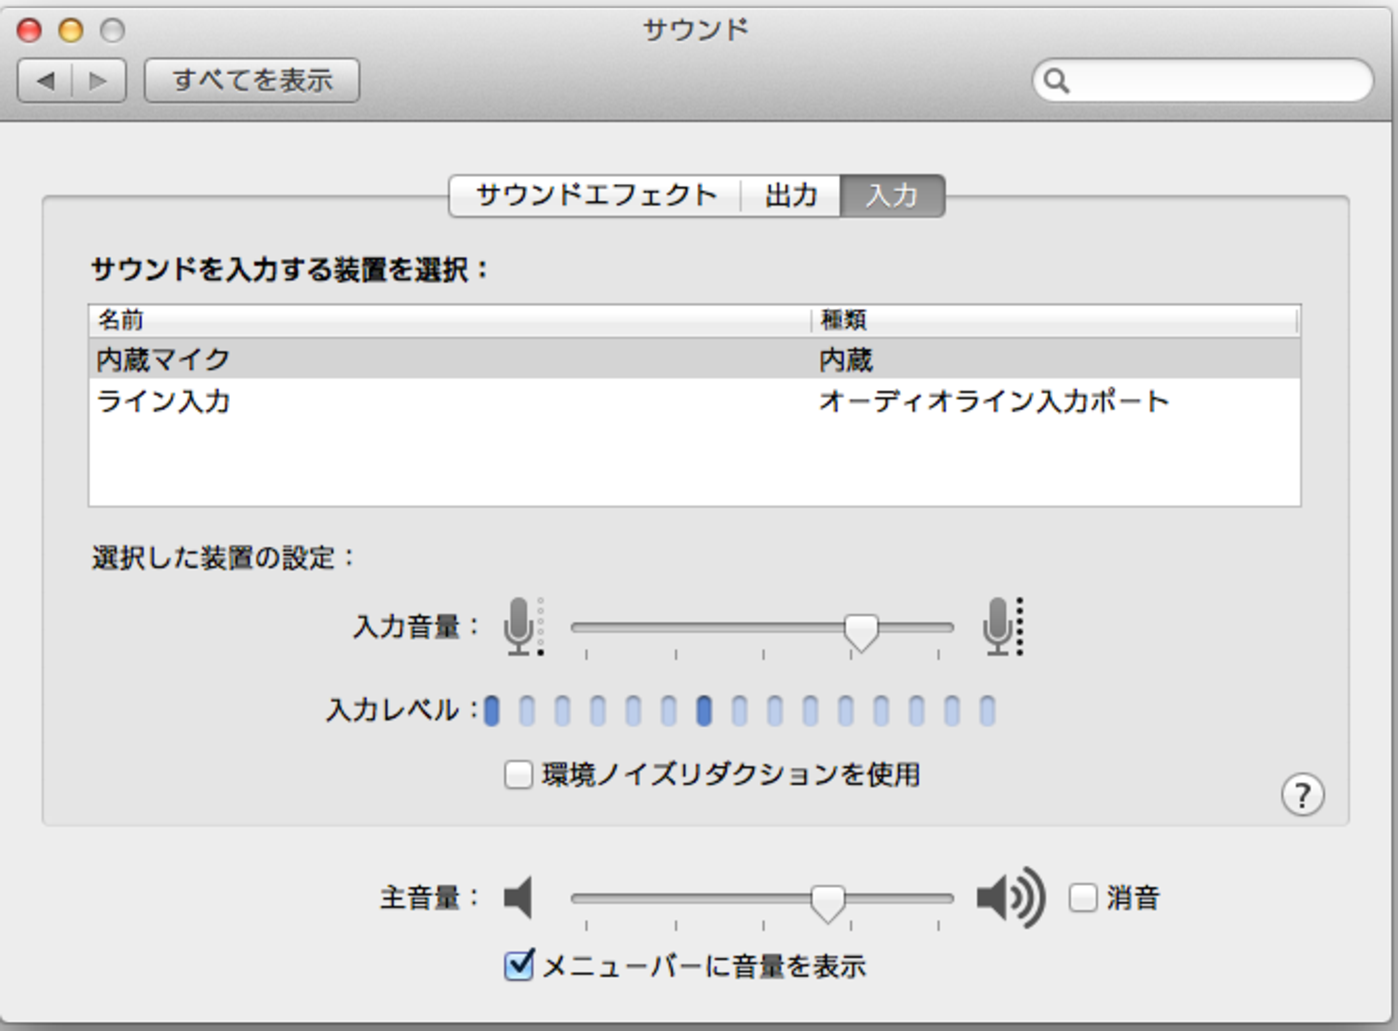
\includegraphics[scale=0.3]{setting.pdf}
	\end{center}
	\caption{Macのサウンドの設定}
	\label{fig:internal_mic}
\end{figure}

\begin{figure}

\end{figure}
前回までは、SCを用いて音を生成する方法を学習してきたが、今回はマイクからの入力音をリアルタイムに加工する方法に焦点をあて、リング・モジュレーション、ディストーション、ピッチ・シフター、ディレイ、リバーブなどのエフェクトの作成をオムニバス的に紹介していく。ハウリングを避けるために、本稿のプログラムを実行する際には、ヘッドフォンなどを着用すること。また、OS側の設定で必ずマイクがオーディオ入力機器に選択されていることを事前に確認すること。Macの場合は、図\ref{fig:internal_mic}のように、「環境設定」パネルの「サウンド」で内蔵マイクをOSのサウンド入力装置として設定し、SCサーバーの起動時にリスト\ref{code:device_list}のように、内蔵マイク入力(Built-in Microphone)がリストの最初に列挙されているのを確認する。

\begin{lstlisting}[caption=入出力デバイスのリスト,label=code:device_list]
Number of Devices: 3
   0 : "Built-in Microph"
   1 : "Built-in Input"
   2 : "Built-in Output"
\end{lstlisting}

\section{マイクからの入力音を得るには}
マイクからの入力をSCで得るには、リスト\ref{code:mic_input}のように{\bf SoundIn}というUGenを用いる。このプログラムでは単純にマイクからの音声をオーディオ出力装置に送っている。プログラムを実行すると、内蔵マイクに拾われた音がそのままヘッドフォンから聞こえてくる。

\begin{lstlisting}[caption=マイク入力,label=code:mic_input]
{
	a = SoundIn.ar(0);
	[a, a];
}.play;
\end{lstlisting}

リストでは、SoundInの引数として「0」という数値が与えられているが、これは最初のオーディオ入力チャンネル、すなわちコンピュータのステレオ・マイクのLチャンネルを取得するという意味である。もし、「0」のかわりに[0,1]のようにArrayを与えると左右両方のチャンネルを取得することができる。また、3行目の[a, a]というArrayは単純にヘッドフォンの左右両方のチャンネルにマイクからの音を送るためのものである。このかわりにもし、「a」のみを書いた場合は、ヘッドフォンの左チャンネルのみにしか音が送られない。
\begin{itembox}[l]{SoundIn}
{\footnotesize 
コンピュータのマイクやサウンドカードからの音声入力を得る\\
.ar({\it bus}, {\it mul}, {\it add})\\
{\it bus}$\cdots$入力チャンネル番号。Arrayを与えることで、複数のチャンネルを同時に取得可能\\
}
\end{itembox}

\section{リング・モジュレーション}
まず初めに、単純なエフェクトの一例として、リング・モジュレーションをプログラムする。リング・モジュレーションは入力音の周波数成分の周囲にサイドバンドと呼ばれる周波数成分を作り出して入力音の音色を変化させるもので、リスト\ref{code:rm}のように、SoundInからの入力音に正弦波を掛けあわせてプログラムする事ができる。

\begin{lstlisting}[caption=リング・モジュレーション,label=code:rm]
{
	a = SoundIn.ar(0) * SinOsc.ar(MouseX.kr(20,880));
	[a, a];
}.play;
\end{lstlisting}

リストでは、MouseXを用いてカーソルの画面上の位置で正弦波の周波数をコントロールできるようにしている。

\section{ディストーション}
オーディオ信号を増幅し歪ませる事で、豊かな倍音を含んだ太い音を得る、ロック・ギターでお馴染みのディストーションはSC3ではリスト
\ref{code:dst}のように.distortメソッドを用いてプログラムする事ができる。

\begin{lstlisting}[caption=ディストーション, label=code:dst]
{
	a = SoundIn.ar(0, 100).distort * 0.1;
	[a, a];
}.play;
\end{lstlisting}

.distortを用いて確実に入力音を歪ませるには、ある程度の振幅のある入力音が必要となる。
このため、リストではSoundInの{\it mul}引数を100に設定して入力音を100倍に増幅し、.distortにより歪ませた後、「* 0.1」で聴取しやすいよう、レベルの調整をしている。
.distortの他にも.softclipを使うと.distortと違った歪み方をさせることが可能である。図\ref{fig:comparison}は10倍に増幅した正弦波をそれぞれ.softclipと.distortで歪ませた時の波形の違いを図示したものである。

\begin{figure}[htbp]
	\begin{center}
		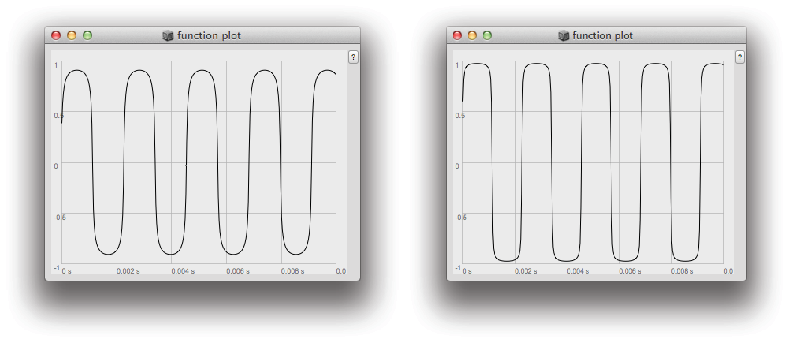
\includegraphics[scale=0.6]{comparison.pdf}
	\end{center}
	\caption{.distort(左)と.softclip(右)により歪ませた正弦波}
	\label{fig:comparison}
\end{figure}

\section{ピッチ・シフター}
入力音のピッチを自在に変化させるピッチ・シフターは{\bf PitchShift}というUGenを用いれば簡単にプログラム可能である。PitchShiftはごく短いバッファに入力音を繰り返し録音し、それを{\it pitchRatio}パラメータで指定された速度で再生することにより入力音の音程を変化させている。リスト\ref{code:ps}では、このパラメータを0.5に設定しているため、入力音が半分の速度での再生される、このため入力音を1オクターブ低くシフトした音が作られる。

\begin{lstlisting}[caption=ピッチ・シフター, label=code:ps]
{
	a = PitchShift.ar(SoundIn.ar(0), pitchRatio:0.5);
	[a, a];
}.play;
\end{lstlisting}

例えば、原音より短三度高い音と長三度低い音を付加してピッチ・シフターを利用した和音を作る事も可能である。このように音階上にピッチシフトを行う場合は、以前に学習した.midicpsを利用する。

\begin{lstlisting}[caption=ピッチ・シフターによる和音, label=code:ps_chord]
{
	a = PitchShift.ar(SoundIn.ar([0,1]), pitchRatio: 3.midicps / 0.midicps);
	a = PitchShift.ar(SoundIn.ar([0,1]), pitchRatio: -4.midicps / 0.midicps) + a;
	[a, a];
}.play;
\end{lstlisting}

.midicpsは、MIDIノートナンバーを周波数に変換するメソッドであり。「0.midicps」を実行すると、MIDIノートナンバー「0」の周波数を得られる。MIDIノートナンバー「0」より長三度高い、つまり半音階で4高いMIDIノートナンバー「4」と、短三度低い、つまり半音階で3低い、ノートナンバー「-3」の周波数をそれぞれもとめ、それをノートナンバー「0」の周波数で除算することで、ノートナンバー「4」と「-3」と「0」間の周波数比、つまりどれだけ速く(あるいは遅く)入力音を再生すれば、その音程が得られるかが数値として得る事ができる。これを{\it pitchRatio}の値としてPitchShift.arに与える事で、入力音より短三度高い音と長三度低い音を作り、ピッチ・シフターを用いた長三和音を実現する事ができる。

\begin{itembox}[l]{PitchShift}
{\footnotesize 
ピッチシフトを行うUGen。音程は{\it pitchRatio}で指定する。dispersionのパラメータを用いることで、音程のランダマイズなども可能。\\
.ar({\it in}, {\it windowSize}, {\it pitchRatio}, {\it pitchDispersion}, {\it timeDispersion}, {\it mul}, {\it add}, )\\

{\it in}$\cdots$入力信号\\
{\it windowSize}$\cdots$ウインドウ・サイズ\\
{\it pitchRatio} $\cdots$ピッチ・レシオ。再生速度\\
{\it pitchDispersion} $\cdots$ピッチ分散度\\
{\it timeDispersion} $\cdots$時間分散度\\
}
\end{itembox}

\section{ディレイ}
本項では入力音を一定時間遅延させるディレイとその応用を数種紹介する。

\subsection{シンプルなディレイ}

遅延効果をSCで用いるには{\bf DelayN}というUGenを使用する。このUGenの第2、第3引数はそれぞれ、最大ディレイ・タイム最大({\it maxdelaytime})とディレイ・タイム({\it delaytime})で、最大ディレイ・タイムの値を元にSCはディレイ用のバッファを用意し、それを利用してディレイ・タイムで指定された時間だけ入力音を遅延させて出力する。最大ディレイ・タイムを超えたディレイ・タイムを設定した場合、ディレイ・タイムは最大ディレイ・タイムにクリップされる(リスト\ref{code:delay})。
\begin{lstlisting}[caption=ディレイ, label=code:delay]
{
	a = DelayN.ar(SoundIn.ar(0), 0.5, 0.5)
	[a, a];
}.play;
\end{lstlisting}

\begin{itembox}[l]{DelayN}
	{\footnotesize 
	入力音を{\it delaytime}で指定した時間だけ遅延させる。\\
	.ar({\it in}, {\it maxdelaytime}, {\it delaytime}, {\it mul}, {\it add})\\
	{\it in}$\cdots$入力信号。\\
	{\it maxdelaytime}$\cdots$最大ディレイ・タイム。ディレイ用のバッファの確保に使用する。\\
	{\it delaytime} $\cdots$ディレイ・タイム。最大ディレイ・タイムより大きい値を指定した場合、最大ディレイ・タイムにクリップされる。
	}
\end{itembox}

\subsection{フィードバック・ディレイ}
\begin{figure}[htbp]
	\begin{center}
		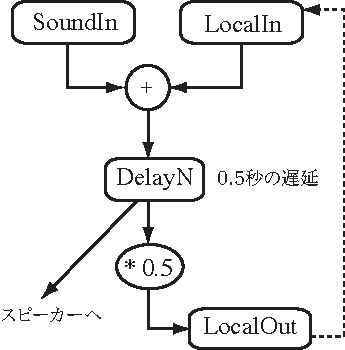
\includegraphics[scale=0.7]{feedback.pdf}
	\end{center}
	\caption{フィードバック・ディレイの成り立ち}
	\label{fig:feedback}
\end{figure}

遅延させた信号を振幅を弱め、もう一度Delay.arに入力することによって、入力音が減衰しながらも何度も繰り返される、やまびこのようなエフェクト、フィードバック・ディレイが実現できる(図\ref{fig:feedback})。このようなフィードバック・ディレイを実現するには、リスト\ref{code:feedback}のように{\bf LocalIn}と{\bf LocalOut}というUGenを用いる。リストでは、4行目でDelayNによる0.5秒の遅延処理と「* 0.5」による振幅の減衰が施された信号をLocalOutに送り、それが2行目のLocalInによって取り出され、原音と加算されている。LocalOutの引数としてオーディオ信号のArrayを渡す事で、複数のチャンネルをLocalOutに送る事も可能であり。複数のチャンネルをLocalOutに送った場合は、2行目のように、そのチャンネル数(= 2)をLocalInの第1引数として指定する。

\begin{lstlisting}[caption=フィードバック・ディレイ, label=code:feedback]
{
	a = SoundIn.ar([0,1]) + LocalIn.ar(2);
	d = DelayN.ar(a, 0.5, 0.5);
	LocalOut.ar(d*0.5);
	[d, d]
}.play
\end{lstlisting}

\subsection{ピンポン・ディレイ}
フィードバック・ディレイにアレンジを加え、各ディレイ音が左右のスピーカーから交互に聞こえる、ピンポン・ディレイを作る事もできる。

\begin{figure}[htbp]
	\begin{center}
		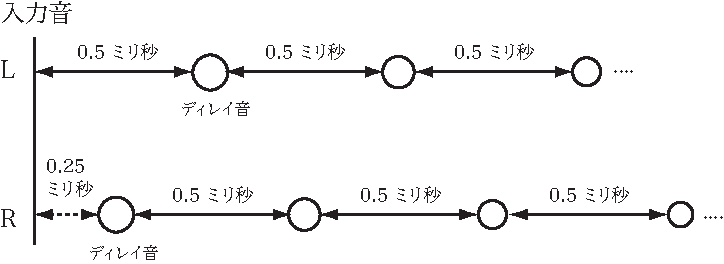
\includegraphics[scale=0.65]{pingpong.pdf}
	\end{center}
	\caption{ピンポンディレイ}
	\label{fig:pingpong}
\end{figure}

左右のスピーカーに交互にディレイを送るには左右のスピーカー用にそれぞれ独立したフィードバック・ディレイを用意し、片方のスピーカーのフィードバック・ディレイに音を入力するタイミイングをもう片方に入力するタイミングとずらすことにより実現できる(図\ref{fig:pingpong})。

リスト\ref{code:pp}は0.25秒ごとに左右のスピーカーから交互にディレイ音が聞こえるピンポン・ディレイのプログラム例である。3行目では、入力音に0.25秒の遅延と「* 0.8」により振幅を減衰を施し、それを変数dに代入している。また、4行目でLocalInを用いてLocalOutからの2チャンネルの信号を取得し、変数lに代入。5、6行目でLチャンネルを入力音(a[0])と、Rチャンネル(a[1])を0.25秒の遅延を伴った、dとミックスしている。それを、7、8行目で、それぞれ個別のDelayNに入力することによって、0.5秒さらに遅延させ、9行目でLocalOutに送り、フィードバックを生じさせている。10行目には[l,r+d]となっているため、左のスピーカーからはl音、つまり0.5、1.0、1.5、2.0...秒後にディレイが聞こえ、右のスピーカーかrとdの音のミックスしたrの音、つまり0.25、0.75、1.25、1.75...秒後にディレイが聞こえてくる。

\begin{lstlisting}[caption=ピンポン・ディレイ, label=code:pp]
{
	i = SoundIn.ar(0);
	d = DelayN.ar(i, 0.25, 0.25) * 0.8;
	a = LocalIn.ar(2);
	l = a[0] + i;
	r = a[1] + d;
	l = DelayN.ar(l, 0.5, 0.5) * 0.8; 
	r = DelayN.ar(r, 0.5, 0.5) * 0.8;
	LocalOut.ar([l,r]);
	[l,r+d]
}.play
\end{lstlisting}

\subsection{マルチタップ・ディレイ}
リスト\ref{code:multitap}のようにDelayNとArrayと組み合わせて、リズミカルなディレイ(=マルチタップ・ディレイ)を作る事も可能である。

\begin{lstlisting}[caption=マルチタップ・ディレイ, label=code:multitap]
{
	t = 0.1;
	a = [1, 2, 4, 6, 7] * t;
	d = DelayN.ar(SoundIn.ar(0), a, a);
	[d, d];
}.play
\end{lstlisting}

このリストで変数aはマルチタップ・ディレイのリズムパターンが定義されたArrayが格納されている。Arrayは[1, 2, 4, 6, 7]というリズムパターンに0.1が掛けられているので、その内容は[0.1, 0.2, 0.4, 0.6, 0.7]となる、このArrayを4、5行目のDelayNの最大ディレイ・タイムとディレイ・タイムにそれぞれ適応している。このように引数にArrayが与えられた場合、SCは自動的にDelayNを複製する(図\ref{fig:multitap})。

\begin{figure}[htbp]
	\begin{center}
		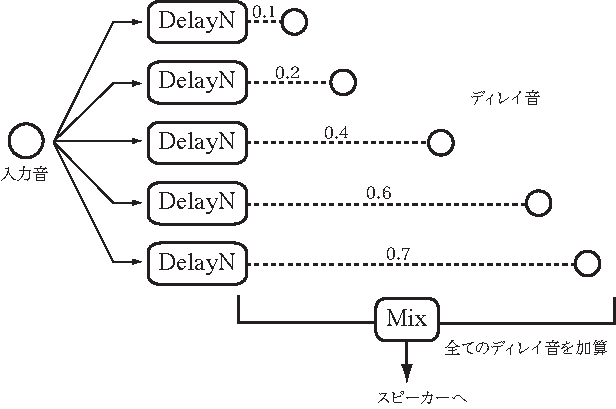
\includegraphics[scale=0.7]{multitap.pdf}
	\end{center}
	\caption{マルチタップ・ディレイ}
	\label{fig:multitap}
\end{figure}

ここでは5つの要素からなるArrayが与えられたため、DelayNが5つ作られ、それぞれに異なった最大ディレイ・タイム及びディレイ・タイムが指定される。この全てのDelayNからの出力は5つの要素を持つArrayとして4、5行目でチャンネルごとに変数l、rに格納される。そして、6行目で{\bf Mix}というUGenを使って、Array内の全てをミックスしている。2行目の変数tを変更する事で、リズムを保持したまま、テンポだけを変える事が可能である。

\begin{itembox}[l]{Mix}
{\footnotesize 
{\it array}内の音声信号を全て加算する\\
.ar({\it array})\\
{\it array}$\cdots$音声信号のArray、全てのチャンネルが加算される\\
}
\end{itembox}

ディレイは非常に多様な可能性を持っており、本項で紹介したような純粋な遅延効果の他にも、フランジャーやコーラスのようなエフェクトをこれを応用して作る事ができる。これらについてはまた回を改めて紹介する。

\section{リバーブ}
残響効果を入力音に加えるには、以下のようにFreeVerbというUGenを利用するのが最も簡単である。

\begin{lstlisting}[caption=リバーブ, label=code:reverb]
{
	FreeVerb.ar(SoundIn.ar([0,1]), 1.0);
}.play
\end{lstlisting}

\begin{itembox}[l]{FreeVerb}
{\footnotesize 
原音にリバーブ(残響効果)を付加するUGen\\
.ar({\it in}, {\it mix}, {\it room}, {\it damp}, {\it mul}, {\it add})\\
{\it in}$\cdots$入力信号\\
{\it mix}$\cdots$原音と加工音のバランス、1で加工音のみ、0で原音のみ\\
{\it room} $\cdots$ルームサイズ、1.0が最大、0.0が最小\\
{\it damp} $\cdots$高周波数のダンプ。0から1の範囲で指定\\
}
\end{itembox}

\section{フィルタ}
SCには様々なフィルタが予め用意されている。リスト\ref{code:highpass}では、入力音にハイパス・フィルタを施し、3000Hz以下の低周波成分を減衰させている。

\begin{lstlisting}[caption=ハイパス・フィルタ, label=code:highpass]
{
	a = HPF.ar(SoundIn.ar(0), 3000);
	[a, a];
}.play;
\end{lstlisting}

SCにはHPF(High Pass Filter) の他にもLPF(Low Pass Filter)、BPF(Band Pass Filter)、Moog、TwoPoleなど様々なフィルタが用意されている。「Filter」をヘルプで調べると、全てのフィルタのリストを見ることができる。

\begin{itembox}[l]{HPF}
{\footnotesize 
2次バターワース・ハイパスフィルタ\\
.ar({\it in}, {\it freq}, {\it mul}, {\it add})\\

{\it in}$\cdots$入力信号\\
{\it freq}$\cdots$カットオフ周波数\\
}
\end{itembox}

\section{ワウワウ}
リスト\ref{code:wahwah}では、バンド・パスフィルタ中央周波数のパラメータをLFOでコントロールすることにより、ファンク・ギターなどでお馴染みの「ワウワウ」のエフェクトを作成している。
\begin{lstlisting}[caption=ワウワウ, label=code:wahwah]
{
	l = SinOsc.ar(5, 0, 1000, 1500);
	a = BPF.ar(SoundIn.ar([0,1]), l, 0.5);
	[a, a];
}.play;
\end{lstlisting}

BPFの三番目の引数はrq(reciprocal of Q)値であり、この値が少なければ少ないほどフィルタを通過する帯域幅が狭くなり、強くワウワウがかかる。

\begin{itembox}[l]{BPF}
{\footnotesize 
2次バターワース・バンドパスフィルタ\\
.ar({\it in}, {\it freq}, {\it rq}, {\it mul}, {\it add})\\

{\it in}$\cdots$入力信号\\
{\it freq}$\cdots$中央周波数\\
{\it rq}$\cdots$reciprocal of Q値\\
}
\end{itembox}

\section{エフェクタをSynthDefとしての定義する}
SC3はこれまでに制作してきたようなエフェクタを複数組み合わせ、SynthDefとして定義することも可能である。リスト\ref{code:combination}ではピッチ・シフター・ディレイ・リバーブを連結して、より複雑なエフェクトをプログラムし、それを「myEffect」というSynthDefとして定義している。

\begin{lstlisting}[caption=エフェクトの組み合わせ, label=code:combination]
SynthDef("myEffect",{
	i = SoundIn.ar([0,1]);
	i = PitchShift.ar(i, pitchRatio:0.5) + i;
	i = DelayN.ar(i, 0.5, 0.5) + i;
	i = FreeVerb.ar(i, 1.0) + i;
	Out.ar(0, [i, i]);
}).load;

Synth("myEffect")
\end{lstlisting}

リストでは3から5行目にかけて、「+ i」が行末に書かれているが、これはエフェクトにより加工された音と、エフェクトへの入力音を足し、両方の音が聞こえるようにするためである。

\section{まとめ}
今回はSCによる様々なエフェクトのプログラミングを学習した。エフェクタは、さらにSCのバス(Bus)と言われる機能を利用して、エフェクタのSynthを複数繋ぐ、音を生成するSynthとエフェクタを定義したSynthを組み合わせて、自作シンセ音に各種エフェクトを
適応するという等、様々な応用が可能である。このバス機能については、また回を改めて紹介する。

\bibliographystyle{jplain}
\begin{thebibliography}{citations}
  \bibitem{scsite} {\it SuperCollider}, \url{http://supercollider.sourceforge.net}(アクセス日 2014年6月10日)
\end{thebibliography}

\section{著者プロフィール}
\subsection{美山 千香士 (Chikashi Miyama)}
作曲家、電子楽器創作家、映像作家、パフォーマー。国立音楽大学音楽デザイン学科より学士・修士を、スイス・バーゼル音楽アカデミーよりナッハ・ディプロムを、アメリカ・ニューヨーク州立バッファロー大学から博士号を取得。作曲・コンピュータ音楽を莱孝之、エリック・オニャ、コート・リッピ氏らに師事。Prix Destellos特別賞、ASCAP/SEAMUS委嘱コンクール2位、ニューヨーク州立大学学府総長賞、国際コンピュータ音楽協会賞を受賞。2004年より作品と論文が国際コンピュータ音楽会議に13回入選、現在までに世界19カ国で作品発表を行っている。 2011年、DAAD(ドイツ学術交流会)から研究奨学金を授与され、ドイツ・カールスルーエのZKMで客員芸術家として創作活動に従事。近著に「Pure Data-チュートリアル&リファレンス」(Works Corporation 社)がある。現在ドイツ・ケルン音楽大学講師。スイス・チューリッヒ芸術大学コンピュータ音楽・音響研究所(ICST)研究員。バーゼル造形大学のプロジェクト「Experimental Data Aesthetics」プログラマ。2013年に松村誠一郎氏と日本語のPure Data ポータル Pure Data Japan(\url{http://puredatajapan.info})を創設。公式ウェブサイト:\url{http://chikashi.net}
\end{document}
